\question[7] Consider the non-linear system below.  
\begin{align*}
    \dxdt &= (x-4)(y-3) , \qquad \dydt = x-y^2
\end{align*}
\begin{parts}
\part Sketch the nullclines of the system on the axes below. Clearly indicate the critical points.
    \ifnum \Solutions=1 {\color{DarkBlue} \\[12pt] 
    Green curves are the $x-$nullclines, black curves are the $y-$nullclines.
    \begin{center}
    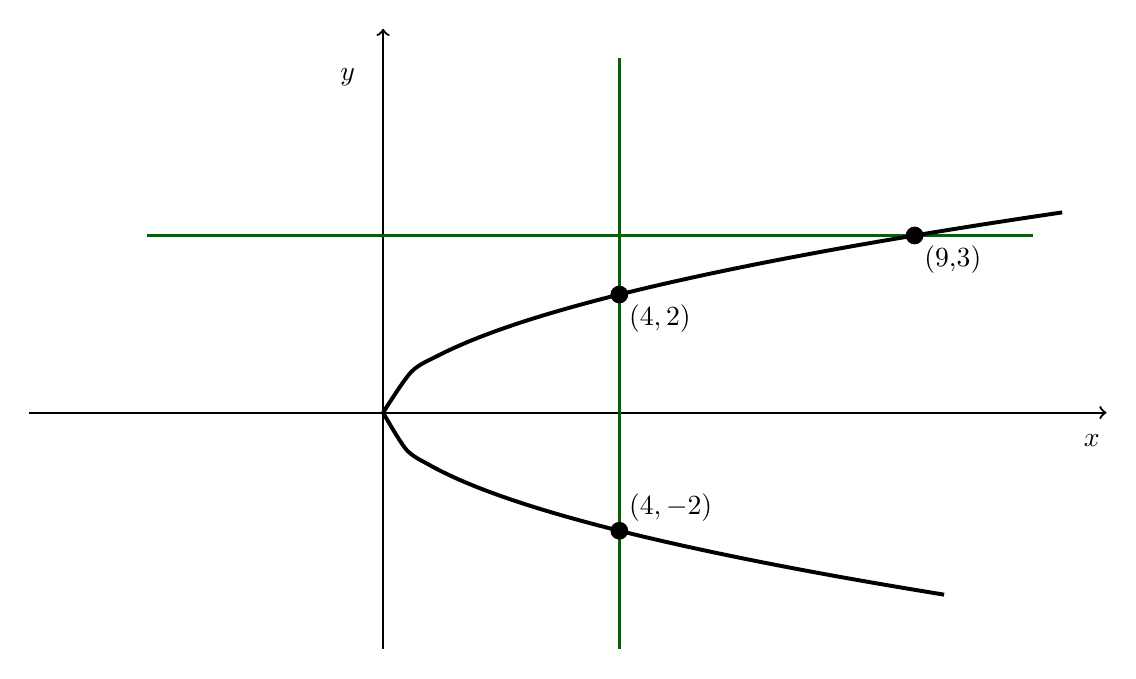
\begin{tikzpicture}[scale=0.75]
    \draw[thick, ->] (-6, 0) -- (12.25, 0);
    \draw[thick, ->] (0, -4) -- (0, 6.5);
    \node[overlay, below] at (12, -0.2) {$x$};
    \node[overlay, below] at (-0.6, 6) {$y$};   
    \draw[very thick,DarkGreen, -] (4, 6) -- (4, -4);        
    \draw[very thick,DarkGreen, -] (-4, 3) -- (11, 3);   
    \draw[black, line width = 0.50mm]   plot[smooth,domain=0:11.5] (\x, {\x^(1/2)});
    \draw[black, line width = 0.50mm]   plot[smooth,domain=0:9.5] (\x, {-sqrt(\x)});
    \filldraw[black] (4,2) circle (4pt) node[anchor=north west]{$(4,2)$};
    \filldraw[black] (4,-2) circle (4pt) node[anchor=south west]{$(4,-2)$};
    \filldraw[black] (9,3) circle (4pt) node[anchor=north west]{(9,3)};
    \end{tikzpicture}
    \end{center}            
    } 
    \else 
    \begin{center}
    \begin{tikzpicture}[scale=0.55]
    \draw[very thick, ->] (-6, 0) -- (6.25, 0);
    \draw[very thick, ->] (0, -6) -- (0, 6.25);
    \node[overlay, below] at (6, -0.2) {$x$};
    \node[overlay, below] at (-0.6, 6) {$y$};        
    \end{tikzpicture}
    \end{center}    
    \fi
    \part Determine the locations of the critical points. 
    \ifnum \Solutions=1 {\color{DarkBlue} \\[12pt] 
    Setting both $x'=0$ and $y'=0$, we obtain three critical points as follows. 
    
    Setting $x'=0$ implies $y=3$ or $x=4$. 
        \begin{itemize}
            \item If $y=3$, then for $y'=0$ we need $x=9$. There is a CP at $(9,3)$. 
            \item If $x=4$, then for $y'=0$ we solve $4 = y^2$. So there are CPs at $(4,\pm2)$.
        \end{itemize}
        The CPs are located at $(9,3)$ and $(4,\pm2)$.
        } 
    \else 
    \vfill
    \fi
\end{parts}
